\documentclass[letterpaper,12pt,oneside]{article}\usepackage[]{graphicx}\usepackage[]{color}
%% maxwidth is the original width if it is less than linewidth
%% otherwise use linewidth (to make sure the graphics do not exceed the margin)
\makeatletter
\def\maxwidth{ %
  \ifdim\Gin@nat@width>\linewidth
    \linewidth
  \else
    \Gin@nat@width
  \fi
}
\makeatother

\definecolor{fgcolor}{rgb}{0.345, 0.345, 0.345}
\newcommand{\hlnum}[1]{\textcolor[rgb]{0.686,0.059,0.569}{#1}}%
\newcommand{\hlstr}[1]{\textcolor[rgb]{0.192,0.494,0.8}{#1}}%
\newcommand{\hlcom}[1]{\textcolor[rgb]{0.678,0.584,0.686}{\textit{#1}}}%
\newcommand{\hlopt}[1]{\textcolor[rgb]{0,0,0}{#1}}%
\newcommand{\hlstd}[1]{\textcolor[rgb]{0.345,0.345,0.345}{#1}}%
\newcommand{\hlkwa}[1]{\textcolor[rgb]{0.161,0.373,0.58}{\textbf{#1}}}%
\newcommand{\hlkwb}[1]{\textcolor[rgb]{0.69,0.353,0.396}{#1}}%
\newcommand{\hlkwc}[1]{\textcolor[rgb]{0.333,0.667,0.333}{#1}}%
\newcommand{\hlkwd}[1]{\textcolor[rgb]{0.737,0.353,0.396}{\textbf{#1}}}%

\usepackage{framed}
\makeatletter
\newenvironment{kframe}{%
 \def\at@end@of@kframe{}%
 \ifinner\ifhmode%
  \def\at@end@of@kframe{\end{minipage}}%
  \begin{minipage}{\columnwidth}%
 \fi\fi%
 \def\FrameCommand##1{\hskip\@totalleftmargin \hskip-\fboxsep
 \colorbox{shadecolor}{##1}\hskip-\fboxsep
     % There is no \\@totalrightmargin, so:
     \hskip-\linewidth \hskip-\@totalleftmargin \hskip\columnwidth}%
 \MakeFramed {\advance\hsize-\width
   \@totalleftmargin\z@ \linewidth\hsize
   \@setminipage}}%
 {\par\unskip\endMakeFramed%
 \at@end@of@kframe}
\makeatother

\definecolor{shadecolor}{rgb}{.97, .97, .97}
\definecolor{messagecolor}{rgb}{0, 0, 0}
\definecolor{warningcolor}{rgb}{1, 0, 1}
\definecolor{errorcolor}{rgb}{1, 0, 0}
\newenvironment{knitrout}{}{} % an empty environment to be redefined in TeX

\usepackage{alltt}
\usepackage[paperwidth=8.5in,paperheight=11in,top=1in,bottom=1in,left=1in,right=1in]{geometry}
\usepackage{setspace}
% \usepackage[colorlinks=true,allcolors=Blue]{hyperref}
\usepackage[hidelinks]{hyperref}
\usepackage[usenames,dvipsnames]{xcolor}
\usepackage{indentfirst}
\usepackage{titlesec}
\usepackage{multirow}
\usepackage{booktabs}
\usepackage{graphicx}
\usepackage{verbatim}
\usepackage{rotating}
\usepackage{tabularx}
\usepackage{outlines}
\usepackage{lineno}
\usepackage{array}
\usepackage{times}
\usepackage{cleveref}
\usepackage{acronym}
\usepackage[position=t]{subfig}
\usepackage{paralist}
\usepackage[noae]{Sweave}
\usepackage{natbib}
\usepackage{array}
\usepackage{pdflscape}
\usepackage{bm}
% \usepackage{showlabels}
\bibpunct{(}{)}{;}{a}{}{,}

% page margins and section title formatting
\linespread{1.5}
\setlength{\footskip}{0.5in}
\titleformat*{\section}{\Large\bf\em}
\titleformat*{\subsection}{\singlespace\large\bf}
\titleformat*{\subsubsection}{\singlespace\normalsize\bf\em}
\titlespacing{\section}{0in}{0in}{0in}
\titlespacing{\subsection}{0in}{0in}{0in}
\titlespacing{\subsubsection}{0in}{0in}{0in}

% cleveref options
\crefname{table}{Table}{Tables}
\crefname{figure}{Fig.}{Figs.}
\renewcommand{\figurename}{Fig.}

% aliased citations
\defcitealias{CDMO14}{CDMO 2014}
\defcitealias{NRC00}{NRC 2000}
\defcitealias{RDCT14}{RDCT 2014}

% acronyms
\acrodef{DO}[DO]{dissolved oxygen}
\acrodef{EPA}[EPA]{Environmental Protection Agency}
\acrodef{NERRS}[NERRS]{National Estuarine Research Reserve System}
\acrodef{RMSE}[RMSE]{root mean square error}
\acrodef{SWMP}[SWMP]{System Wide Monitoring Program}
\acrodef{WRTDS}[WRTDS]{weighted regression on time, discharge, and season}

% assorted functions
% for multiple rows in table headers
\newcommand{\head}[2]{\multicolumn{1}{>{\arraybackslash}p{#1}}{#2}}
% for milligrams per litre
\newcommand{\mgl}{mg L$^{-1}$}

% hides (not removes) numbering for section, subsection, etc.
% left indents
\renewcommand{\thesection}{}
\renewcommand{\thesubsection}{}
\renewcommand{\thesubsubsection}{}
\makeatletter
\def\@seccntformat#1{\csname #1ignore\expandafter\endcsname\csname the#1\endcsname\quad}
\let\sectionignore\@gobbletwo
\def\@subseccntformat#1{\csname #1ignore\expandafter\endcsname\csname the#1\endcsname\quad}
\let\subsectionignore\@gobbletwo
\def\@subsubseccntformat#1{\csname #1ignore\expandafter\endcsname\csname the#1\endcsname\quad}
\let\subsubsectionignore\@gobbletwo
\let\latex@numberline\numberline
\def\numberline#1{\if\relax#1\relax\else\latex@numberline{#1}\fi}
\makeatother

% dependent data



%knitr options


\IfFileExists{upquote.sty}{\usepackage{upquote}}{}
\begin{document}

\raggedbottom
\linenumbers
\raggedright
\urlstyle{same}
\setlength{\parindent}{0.5in}
\renewcommand\refname{References \vspace{12pt}}

%%%%%%
% title page
\begin{singlespace}
\title{{\bf {\Large Improving estimates of ecosystem metabolism by removing effects of tidal advection in dissolved oxygen time series}}}
\author{
  {\bf {\normalsize Marcus W. Beck$^1$, Michael C. Murrell$^2$, James D. Hagy III$^2$}}
  \\\\{\textit {\normalsize $^1$ORISE Research Participation Program}}
  \\{\textit {\normalsize USEPA National Health and Environmental Effects Research Laboratory}}
	\\{\textit {\normalsize Gulf Ecology Division, 1 Sabine Island Drive, Gulf Breeze, FL 32561}}
	\\{\textit {\normalsize Phone: 850-934-2480, Fax: 850-934-2401, Email: \href{mailto:beck.marcus@epa.gov}{beck.marcus@epa.gov}}}
  \\\\{\textit {\normalsize $^2$USEPA National Health and Environmental Effects Research Laboratory}}
	\\{\textit {\normalsize Gulf Ecology Division, 1 Sabine Island Drive, Gulf Breeze, FL 32561}}
	\\{\textit {\normalsize Phone: 850-934-2433, Fax: 850-934-2401, Email: \href{mailto:murrell.michael@epa.gov}{murrell.michael@epa.gov}}}
  \\\\{\textit {\normalsize $^3$USEPA National Health and Environmental Effects Research Laboratory}}
	\\{\textit {\normalsize Gulf Ecology Division, 1 Sabine Island Drive, Gulf Breeze, FL 32561}}
	\\{\textit {\normalsize Phone: 850-934-2455, Fax: 850-934-2401, Email: \href{mailto:hagy.jim@epa.gov}{hagy.jim@epa.gov}}}
	}
\date{}
\maketitle
\vfill{\centerline{\textit {\normalsize Running head: Improving Estimates of Estuary Metabolism}}}
\end{singlespace}
\clearpage

%%%%%%
% acknowledgments
\section{Acknowledgments}

We acknowledge the significant efforts of research staff and field crews from the \acl{SWMP} of the \acl{NERRS} for providing access to high quality data sets.  We thank Dr. Jane Caffrey and Dr. Erik Smith for reviewing early drafts of the manuscript. The views expressed in this article are those of the authors and do not necessarily reflect the views or policies of the U.S. Environmental Protection Agency.

%%%%%%
% abstract
\newpage
\section{Abstract}


In aquatic ecosystems, time series of \ac{DO} have been used to compute estimates of ecosystem metabolism.  Central to this open water or ``Odum'' method is the assumption that the dissolved oxygen time series is a Lagrangian specification of the flow field.  However, most \ac{DO} time series are collected at fixed locations, such that changes in dissolved oxygen are assumed to reflect metabolism and that effects of advection or mixing can be neglected.  A statistical model using weighted regression was applied to separate variability in \ac{DO} from tidal variation or other advection in estuaries, thereby helping to partially relax this assumption and improve metabolism estimates. The method targets the periodicity of the tidal component while preserving the true biological signal, offering a distinct advantage over traditional deconvulution methods.  The model was developed and tested using simulated \ac{DO} time series with known biological and physical components, and then applied to one year of continuous monitoring data from four stations within the \acl*{NERRS}.  Variability from advection was reduced on average by 70.2\% for production and 74.3\% for respiration.  The model was especially effective when the magnitude of tidal influence was high and correlations between tidal change and the solar cycle were low, whereas collinearity in the latter instance limited model performance. By reducing the effects of physical transport on metabolism estimates, there may be increased potential to empirically relate metabolic rates to causal factors on timescales of several days to several weeks.

\acresetall
\clearpage

%%%%%%
% intro
\section{Introduction} \label{intro}

Ecosystem metabolism describes the balance between production and respiration processes that create and consume organic matter \citep{Kemp12,Needoba12}.  Light exposure experiments of water samples collected at discrete locations and times have traditionally been used to measure metabolic activity \citep{Gaarder27}.  Although highly controlled and precise, bottle-based methods are labor-intensive and not scalable to describe entire ecosystem rates.  Bottle-based methods may also only reliably estimate production and respiration associated with planktonic processes, whereas significant contributions to ecosystem metabolism can arise from other habitats, such as the benthos or intertidal marshes.  By contrast, open-water techniques have been increasingly used to estimate whole system metabolism given the availability of long-term, continuous time series of dissolved oxygen \citep{Odum56,Davanzo96}. Daily integrated measurements of metabolism represent the balance between daytime production and nighttime respiration attributed to all ecosystem components. Open-water estimates also provide a more accessible means of tracking ecosystem change over time as compared to discrete sampling events with bottle-based approaches. Although metabolic rates vary naturally at different spatial and temporal scales \citep{Ziegler98,Caffrey04,Russell07}, anthropogenic nutrient sources are often contributing factors that increase rates of production (\citealt{Nixon95}; \citetalias{NRC00}).  Reliable estimates of whole ecosystem metabolism are critical for measuring both background rates of production and potential impacts of human activities on ecosytem function.     

The ability to accurately estimate whole system metabolism using the open-water method depends on the degree to which assumptions of the theory are satisfied \citep{Staehr10,Kemp12}.  The fundamental assumption is that the time series of \ac{DO} represents a Lagrangian specification of the flow field \citep{Needoba12}.  The Lagrangian specification characterizes an individual fluid parcel through time, such as a parcel of water moving with the tide.  In reality, most \ac{DO} time series are collected at fixed locations such as a mooring or dock, so they are a Eulerian specification of the flow field.  Time series at fixed locations may characterize water masses with different metabolic histories as water is advected past the sensor, leading to errors in metabolism estimates \citep{Kemp80,Russell07}.  Given this critical challenge, the open-water method has been used with varying success in estuaries influenced by tidal transport and mixing \citep{Caffrey04,Russell07,Caffrey14}.  In contrast, the method has been more successfully applied to water quality time series in lakes, although stratification may limit estimates to specific vertical layers \citep{Staehr10,Coloso11,Batt12}. Appropriate placement of monitoring sondes, sampling frequency and duration, and reliability of data from single stations have been relevant issues in applying the open-water method to systems influenced by physical mixing \citep{Russell07,Staehr10}.  Individual sampling stations near bay inlets or along major tidal axes may produce \ac{DO} time series that are strongly influenced by advection, leading to relatively large errors when using the open-water method.   

Although numerous studies have shown that application of the open-water method to lakes or estuaries may be problematic \citep{Ziegler98,Caffrey03,Coloso11,Batt12,Nidzieko14}, very few quantitative approaches have been developed to address potential bias or noise in metabolism estimates resulting from advection.  For example, an extensive analysis by \citet{Caffrey03} applied the open-water method to estimate metabolism at 28 continuous monitoring stations at 14 US estuaries.  A significant portion of the production and respiration estimates were negative (3 - 69\% depending on site), suggesting advection of water masses was a likely a major factor influencing the \ac{DO} time series.  These `anomalous' values are typically omitted from the analysis \citep{Caffrey03,Collins13}, which may upwardly bias estimates of mean metabolism \citep{Caffrey14}.  Further, \citet{Nidzieko14} evaluated the effects of tidal advection on metabolism estimates in a mesotidal estuary.  Estimates from a single location were strongly correlated with the spring-neap cycle such that net heterotrophy was more common during spring tides, whereas metabolism was generally balanced during neap tides.  This example illustrates that metabolism may actually be modulated by the tide, as opposed to artifacts in the \ac{DO} time series caused by advection on daily time scales.  \citet{Nidzieko14} used a control-volume approach by impounding a section of the upper estuary to understand how physical processes contribute to biological variability.  Although useful as an \textit{in situ}, site-specific approach, more accessible statistical methods specific to time series are needed given the increasing availability of continuous monitoring data. For example, \citet{Batt12} explored the use of a Kalman filter \citep{Harvey89} to remove process and observation uncertainty from \ac{DO} time series in lakes.  Similar approaches have not been developed for estuaries, particularly those that address potential effects of tidal advection.

This article describes the development and application of a method for improving estimates of ecosytem metabolism computed from \ac{DO} time series by reducing the effect of tidal advection on continuous \ac{DO} observations.  We used a weighted regression approach originally developed to resolve trends in pollutant concentrations in streams and rivers \citep{Hirsch10}.  The weighted regression approach creates dynamic predictions of \ac{DO} as a function of time and tidal height change, which are then used to filter, or detide, the \ac{DO} signal.  The model is based on the recognition that daily fluctuations in \ac{DO} caused by metabolism are associated with the solar cycle, whereas other fluctuations in estuaries are likely associated with cyclical water level changes that generally exhibit pregression relative to the solar cycle.  The weighted regression model was applied, rather than methods commonly used for detiding in physical oceanography, to allow for the complex and dynamic patterns of \ac{DO} changes relative to advection.  The method targets the periodicity of the tidal component as a separate parameter during model fitting, which allows the ability to isolate the biological component of the dissolved oxygen time series.  As a result, the weighted regression approach can preserve the true biological signal in the output rather than risking removal of both the biological and physical components as with traditional deconvulution methods.  This approach offers a distinct advantage for estuaries where the magnitude of tidal effects on water quality observations can be severe.  During initial method development, we used simulated \ac{DO} time series with known characteristics to evaluate the ability of the weighted regression to remove the simulated effects of a tidally-advected \ac{DO} gradient.  Subsequently, the simulation results informed further development of the method as applied to four case studies chosen from the \aclu{NERRS} (\acs{NERRS}, \citealt{Wenner04}).  In all examples, tidal height is used as a proxy for advection because it was recorded with the \ac{NERRS} data.  In the absence of quantitative data describing lateral \ac{DO} variation (e.g., contemporaneous stations along a tidal axis), the model determines the advective effect empirically.

%%%%%%
% materials and procedures
\section{Materials and Procedures}

\subsection{Weighted regression for modelling and filtering \ac{DO} time series}

For this study, we adapted a weighted regression model to filter \ac{DO} time series for apparent tidal effects.  This model relied heavily on concepts used to develop the \ac{WRTDS} method for estimating pollutant concentrations in streams and rivers \citep{Hirsch10}.  The functional form of the model is:
\begin{equation}\label{funform}
DO_{obs}= \beta_0 + \beta_1 t + \beta_2 H
\end{equation}
where $DO_{obs}$ is a linear function of time $t$ and tidal height $H$.  Time is a continuous variable for the day and time of each observation as a proportion of the number of total observations.  The beginning of each day was defined as the nearest thirty minute observation to sunrise for the location.  Our model differed from the original \ac{WRTDS} method, which included parameters to estimate variation of the response variable on a sinusoidal period.  \ac{DO} variation was not modeled using this approach because the expected metabolically-driven pattern is not strictly sinusoidal.  

Tidal height is used as a proxy for advection because the model is empirical and only requires a variable that is correlated with the true measure of interest.  An important distinction between tidal height and advection is that the two variables could provide different information about a tidal regime.  Tidal heights at the minimum and maximum of the range may be associated with periods of low advection when water masses are not moving rapidly past the sensor, whereas tidal heights near the mean may be more likely to have greater advection.  Accordingly, our use of tidal height should not be confused with a variable that is directly proportional to advection.  The model only requires a variable that indicates a particular point in the tidal cycle, such that tidal height can be mapped to advection with quantifiable periodicity that the model can isolate.  Moreover, tidal height measurements are more widely available and are generally monitored by water quality sondes.    

Weighted regression was implemented as a moving window that allowed for estimation of \ac{DO} throughout the time series by adapting to variation through time as a function of tide. Regression models were estimated sequentially for each observation in the time series using dynamic weight vectors that change with the center of the window.  Weight vectors quantified the relevance of observations to the center of the window in respect to time, hour of the day, and tidal height.  Specifically, weights were assigned to each variable using a tri-cube weighting function \citep{Tukey77,Hirsch10}:
\begin{equation}
w= \left\{ 
  \begin{array}{l l}
    \left(1-\left(d/h\right)^3\right)^3 & \quad \textrm{if } |d| \leq h \\
    0 & \quad \textrm{if } |d| > h 
  \end{array} \right.
\end{equation}
where the weight $w$ of each observation is inversely proportional to the distance $d$ from the center of the window such that observations more similar to the point of reference are given higher weight in the regression.  Observations that exceed the maximum width of the window $h$ are assigned a weight of zero.  The tri-cube weighting function is similar to a Gaussian distribution such that weights decrease gradually from the center until the maximum window width is reached.  Regressions that use simpler windows (e.g., boxcar approach) are  more sensitive to influential observations as they enter or leave the window, whereas the tri-cube function minimizes their effect through gradual weighting of observations from the center \citep{Hirsch10}.  The final weight vector for each observation is the product of the three separate weight vectors for time (day), hour, and tidal height. Windows for time (continuous throughout the day) and hour (within each day) are used to weight observations based on distance (time) from the center of the window.  The window for tidal height is used to weight observations based on the difference from mean tide as a proportion of tide range.  For example, a half-window width of 0.5 means that observations are weighted proportionately within +/- 50\% of the tide range referenced to the tidal height in the center of the window. A low weight is given to an observation if any of the three weighting values were not similar to the center of the window since the final weight vector is the product of three weight vectors for each variable (see the link in the \hyperref[multi]{multimedia} section for graphical display of different weights).    

The choice of window widths for weight vectors affects the model results; therefore, weights were selected via a rational and replicable method.  Window widths that minimize prediction error are typically smaller than widths that should be used to minimize tidal effects.  Similarly, window widths that more effectively filter the \ac{DO} signal may produce less precise predictions for the observed data.  Evaluations of the weighted regression method with simulated \ac{DO} time series, described below, used multiple window widths to evaluate the ability of the model to filter the \ac{DO} signal.  The ability to predict observed \ac{DO} was not a primary objective, rather the window widths were evaluted for their ability to remove tidal variation from the \ac{DO} time series.  

The approach to minimize advection effects in the observed \ac{DO} time series differs slightly from \citet{Hirsch10}, who used a two-dimensional grid predicted for stream pollutant concentrations across the time series and the range of discharge values observed in the study system.  Normalized or discharge-independent values for pollutant concentration were obtained by averaging grid predictions across the discharge values that were likely to occur on a given day.  Rather than creating a two-dimensional grid of \ac{DO} related to time and tidal height change, the normalized time series herein were the model predictions conditional on time and constant tidal height set to the mean:
\begin{equation} \label{do_nrm}
DO_{nrm} = f(DO_{obs}|\bar{H}, t)
\end{equation}
such that the normalized time series represents \ac{DO} variation related to biological processes.  The term `filter' is used in reference to the removal of a specific variance component from the time series, while maintaining the structure of the biological component.  Although the approach shares similarities with common filtering techniques, a distinction is noted such that weighted regression has a specific purpose rather than the more generic objectives of common filters (e.g., moving window averages or local smoothers, \citealt{Shumway11}).     

%%%%%%
% assessment
\section{Assessment}

\subsection{Simulation of \ac{DO} time series}

To test the ability of the weighted regression to filter the \ac{DO} signal for apparent tide effects, multiple time series with known characteristics were simulated and filtered.  A simulation approach was used prior to application with real data because the true biological signal can be specified as a known component for comparison with the filtered results from weighted regression. The following describes the theoretical basis for developing the simulated time series.  Observed \ac{DO} time series ($DO_{obs}$) were simulated as the sum of variation from biological processes ($DO_{bio}$) and physical effects related to tidal advection ($DO_{adv}$):  
\begin{equation} \label{do_obs}
DO_{obs} = DO_{bio} + DO_{adv}
\end{equation}
Each component of $DO_{obs}$ was simulated separately.  The biological \ac{DO} signal ($DO_{bio}$) was the sum of diel variation ($DO_{die}$) plus uncertainty or noise ($DO_{unc}$):
\begin{equation} \label{do_bio} 
DO_{bio} = DO_{die} + DO_{unc}
\end{equation} 
\begin{equation} \label{do_unc}
DO_{unc} = \varepsilon_{obs} + \varepsilon_{pro}
\end{equation}
Biological \ac{DO} signals are inherently noisy \citep{Batt12} such that uncertainty in the biological \ac{DO} signal was described as variation from observation and process uncertainty \citep[$\varepsilon_{obs}$ and $\varepsilon_{pro}$,][]{Hilborn97}. Observation uncertainty is variation related to imprecision in sampling processes or methods, whereas process uncertainty is caused by unknown parameters that contribute to variance in a time-dependent fashion.  For example, wind events can affect air-sea gas exchange \citep{Ziegler98,Caffrey14} such that high wind may contribute to increased process uncertainty.  Although this was not an explicit focus of the simulation analyses, wind effects could be considered an implicit component of process uncertainty in addition to the effects of other unmeasured variables that influence \ac{DO} in a time-dependent manner.  Multiple time series at 30 minute time steps over 30 days were created by varying the relative magnitudes of each of the components of observed \ac{DO} in \cref{do_obs,do_bio,do_unc} to test the effectiveness of weighted regression under different scenarios.  Accordingly, observed \ac{DO} was generalized as the additive combination of four separate time series (\cref{fig:do_sim}):
\begin{equation} \label{do_obs_all}
DO_{obs} = DO_{adv} + DO_{die} + \varepsilon_{obs} + \varepsilon_{pro}
\end{equation} 

Each component of the simulated time series was created as follows.  First, the diel component, $DO_{die}$, was estimated \citep{Cryer08}:
\begin{equation} \label{do_sin}
DO_{die} = \alpha + \beta\cos\left(2\pi ft + \Phi\right)
\end{equation}
such that the mean DO ($\alpha$) was 8, amplitude ($\beta$) was 1, $f$ was 1/48 to represent 30 minute intervals, $t$ was the time series vector and $\Phi$ was the x-axis origin set for an arbitrary sunrise at 630.  The diel signal was increasing during the day and decreasing during the night for each 24 hour period and ranged from 7 to 9 mg L$^{-1}$ (as a general approximation from the case studies below).  Although the representation of $DO_{die}$ as a simple sine wave does not account for lags with the solar cycle or periods of photoinhibition that may be observed in actual time series, we consider the approach sufficient for the simulations.  Uncertainty was added to the diel \ac{DO} signal as the sum of observation and process uncertainty:
\begin{equation} \label{do_unc_n}
DO_{unc, n} = \varepsilon_{obs, n} + \sum_{t = 1}^{n} \varepsilon_{pro, t}
\end{equation}
where observation and process uncertainty ($\varepsilon_{obs}$, $\varepsilon_{pro}$) were simulated as normally distributed random variables with mean zero and standard deviation varying from zero to an upper limit, described below.  Process uncertainty was estimated as a serially correlated variable using the cumulative sum of $n$ observations plus random variation added at each time step for $t = 1, ..., n$.  The total uncertainty, $DO_{unc}$, was added to the diel \ac{DO} time series to create the biological \ac{DO} time series (\cref{do_bio,fig:do_sim}).

A tidal series was simulated based on the principal lunar seimdiurnal (M2) tide with a period of 12.42 hours \citep{Foreman89}.  The amplitude was set to 1 meter and centered  at 4 meters.  The tidal time series simulated \ac{DO} changes with advection, $DO_{adv}$ (\cref{do_obs_all,fig:do_sim}). Conceptually, this vector represents the rate of change in \ac{DO} as a function of horizontal water movement from tidal advection such that:
\begin{equation} \label{deltdo}
\frac{\delta DO_{adv}}{\delta t} = \frac{\delta DO}{\delta x} \cdot \frac{\delta x}{\delta t}
\end{equation}
\begin{equation} \label{deltx}
\frac{\delta x}{\delta t} = a \cdot \frac{\delta H}{\delta t}
\end{equation}
where the first derivative of the tidal time series, as change in height over time $\delta H / \delta t$, is multiplied by a constant $a$, to estimate horizontal tidal excursion over time, $\delta x / \delta t$.  The horizontal excursion is assumed to be associated with a horizontal \ac{DO} change, $\delta DO / \delta x$, such that the product of the two estimates the \ac{DO} change at each time step from advection, $DO_{adv}$. In practice, the simulated tidal signal was used to estimate $DO_{adv}$:
\begin{equation} \label{do_advp}
DO_{adv} = f\left(H\right)
\end{equation}
\begin{equation} \label{do_adv}
DO_{adv} = 2\cdot b + b \cdot \frac{H- \min H}{\max H - \min H}
\end{equation}
where $b$ is analogous to $a$ in \cref{deltx} and is chosen as the transformation parameter to standardize change in \ac{DO} from tidal height change to desired units.  For example, $b = 1$ will convert $H$ to a scale that simulates changes in \ac{DO} from tidal advection that range from +/- 1 mg L$^{-1}$.  The final time series for observed \ac{DO} was the sum of biological \ac{DO} and advection \ac{DO} (\cref{do_obs,fig:do_sim}).

\subsection{Evaluation of weighted regression with simulated \ac{DO} time series}

Multiple time series were simulated by varying the conditions in \cref{do_obs_all} (\cref{fig:sim_ex}) to evaluate weighted regression under a range of conditions. Specifically, the simulated data varied in the relative amount of noise in the measurement ($\varepsilon_{obs}$, $\varepsilon_{pro}$), relative amplitude of the diel \ac{DO} component ($DO_{die}$), and degree of association of the tide with the \ac{DO} signal ($DO_{adv}$).  Three levels were evaluated for each variable: relative noise as 0, 1, and 2 standard deviations for both process and observation uncertainty, amplitude of diel biological \ac{DO} as 0, 1, and 2 mg L$^{-1}$, and \ac{DO} change from tidal advection as 0, 1, and 2 mg L$^{-1}$. A total of 81 time series were created based on the unique combinations of parameters (\cref{fig:sim_ex}).  Half-window widths (day, hour of day, and tide height) for the weighted regressions were evaluated for each time series: time as 1, 3, and 6 days, time of day as 1, 3, and 6 hours, and tidal height as 0.25, 0.5, and 1 as a proportion of the total range given the height at the center of the window.  In total, 27 window width combinations were evaluated for each of 81 simulated time series, producing results for 2,187 weighted regressions.

The filtered \ac{DO} time series were compared to the simulated data to evaluate the ability of weighted regression to characterize the biological \ac{DO} time series in \cref{do_obs}. Comparisons were made using Pearson correlation coefficients and the \ac{RMSE}.  Overall, the weighted regressions produced filtered time series that were comparable to the `true' biological time series regardless of the simulation parameters (\cref{tab:dtd_perf1}) or window widths (\cref{tab:dtd_perf2}, results for each simulation can be viewed using the link in the \hyperref[multi]{multimedia} section).  The median correlation between the filtered and biological values for all time series and window widths was 0.63, with values ranging from 0.05 (very poor) to 1.00 (perfect).  Mean error was 1.02, with values ranging from 0 (perfect) to 2.12 (very poor).  Simulations with very poor performance were those those with the \ac{DO} signal composed entirely of noise from observation uncertainty. As expected, simulations with no biological or tidal influence had filtered time series that were identical to the true time series (e.g., correlation of one, \ac{RMSE} of zero).  

Characteristics of \ac{DO} time series that contributed to improved model performance were increasing amplitude of the diel \ac{DO} component ($DO_{die}$) and increasing process error ($e_{pro}$), whereas increasing observation error contributed to decreased performance (\cref{tab:dtd_perf1,fig:err_surf1}).  Model performance was not significantly affected by increasing tidal effects (i.e., increasing magnitude of $DO_{adv}$).  Model performance was not substantially affected by variation in half window widths relative to characteristics of the \ac{DO} time series (\cref{tab:dtd_perf2,fig:err_surf2}).  Graphical summaries of model performance averaged by simulation parameters (\cref{fig:err_surf1}) and half window widths (\cref{fig:err_surf2}) support the general trends described by \cref{tab:dtd_perf1,tab:dtd_perf2}.

\subsection{Validation of weighted regression with case studies}

Results from the simulated time series were used to inform the validation of weighted regression with real data, specifically with respect to choosing half-window widths described below.  Continuous monitoring data from \ac{NERRS} was used to validate the weighted regression model by evaluating estimates of ecosytem metabolism obtained from observed and filtered \ac{DO} time series. \ac{NERRS} is a network of 28 shallow, productive estuary reserves established for long-term research, water-quality monitoring, education, and coastal stewardship \citep{Wenner04}.  Continuous water quality data have been collected at \ac{NERRS} sites since 1994 through the \aclu{SWMP} (\acs{SWMP}, \citetalias{CDMO14}).  In addition to providing a basis for trend evaluation, data from \ac{SWMP} provides an ideal opportunity to evaluate long-term variation in water quality parameters from biological and physical processes.  Continuous \ac{SWMP} data can be used to describe \ac{DO} variation at sites with different characteristics, including variation from ranges in tidal regime \citep{Sanger02} and rates of ecosystem production \citep{Caffrey03,Caffrey04}.  We selected sites from the \ac{SWMP} database that had desirable characteristics for validating weighted regression.  Specifically, four macrotidal sites were chosen based on apparent relationships between \ac{DO} and tidal changes (\cref{fig:case_map,tab:case_att}).  Moreover, many daily metabolism estimates were not interpretable (i.e., `anomalous') using standard open water methods.  In other words, the advection effects on \ac{DO} time series at these sites are very large.  

The case study sites included Vierra Mouth station at Elkhorn Slough (ELKVM, California, 36.81$^{\circ}$N, 121.78$^{\circ}$W), Bayview Channel at Padilla Bay (PDBBY, Washington, 48.50$^{\circ}$N 122.50$^{\circ}$W), Middle Blackwater River station at Rookery Bay (RKBMB, Florida, 25.93$^{\circ}$N 81.60$^{\circ}$W), and Dean Creek station at Sapelo Island (SAPDC, Georgia, 31.39$^{\circ}$N 81.28$^{\circ}$W).  The ELKVM station is located at the mouth of the Elkhorn Slough estuary in approximately four meters of water (MLW, tidal range 2.0).  Sediments are compacted mud and sand due to large tidal currents.  The PDBBY station is located along the Bayview Channel, which is a major tributary of Padilla Bay that drains intertidal flats that include eelgrass beds and macroalgae.  The site is in 1.5 meters of water (MLLW, tidal range 2.9) with sediments of fine silt and clay overlying sand.  The RKBMB station is located at the mouth of the Middle Blackwater River in approximately 2 meters of water (MHW, tidal range 1.3).  Salinity is oligohaline (2.3 ppt) to polyhaline (38.6 ppt).  Sediments are a mixture of sand, silt, oyster shell, and organic matter.  Finally, the SAPDC station is located in Dean Creek, a small tidal basin that is fed from the Doboy Sound on the south end of Sapelo Island.  Mean low water depth is approximately one meter (tidal range 1.4) and sediments consist of sand and mud with occasional osyter reefs. 

The weighted regression model was applied to continuous \ac{DO} time series and water level measurements from January 1\textsuperscript{st} to December 31\textsuperscript{st} 2012 at the four sites.  \ac{NERRS} sites are typically shallow and vertically-mixed such that one water quality monitor is considered to represent the entire water column, including the benthos.  Tide predictions were obtained for each site using harmonic regression applied to the sonde depth data (\texttt{oce} package in R, \citealt{Foreman89}; \citealt{Kelley14}; \citetalias{RDCT14}). The predicted time series of tidal height from the regressions were used for all models to avoid issues with missing values in the observed data. The stations were generally semidiurnal or mixed semidiurnal and net heterotrophic on an annual basis (\cref{tab:case_att}).

\subsection{Estimates of ecosystem metabolism before and after filtering} \label{met_sec}

The weighted regression method was applied to the annual data for each station to obtain a filtered \ac{DO} time series for estimating metabolism.  Ecosystem metabolism was estimated using the open-water technique \citep{Odum56} as described in \citet{Caffrey14}.  The method is used to infer net ecosystem metabolism using the mass balance equation:
\begin{equation} \label{metrate}
\frac{\delta DO}{\delta t} = P - R + D
\end{equation}
where the change in \ac{DO} concentration ($\delta DO$, g O$_2$ m$^{-3}$) over time ($\delta t$, hours) is equal to photosynthetic rate ($P$, g O$_2$ m$^{-3}$ hr$^{-1}$) minus respiration rate ($R$, g O$_2$ m$^{-3}$ hr$^{-1}$), corrected for air-sea gas exchange ($D$, g O$_2$ m$^{-3}$ hr$^{-1}$) \citep{Caffrey14}. $D$ is estimated as the difference between the \ac{DO} saturation concentration and observed \ac{DO} concentration, multiplied by a volumetric reaeration coefficient, $k_a$ \citep{Thebault08}.  The diffusion-corrected \ac{DO} flux estimates as hourly rates of \ac{DO} change were first averaged during day and night periods for each 24 hour `metabolic day' in the time series. The `metabolic day' was considered the approximate 24 hour period between sunsets on two adjacent calendar days.  Hourly \ac{DO} flux was considered respiration during night hours and net production during day hours.  Total respiration (Rt) rates were assumed constant during day and night such that daily rates were calculated as the average \ac{DO} flux during night hours multiplied by 24. Daily gross production (Pg) was the average \ac{DO} flux during day hours minus the average \ac{DO} flux during night hours, multiplied by total sunlight time.  Net ecosystem metabolism was gross production (positive) plus total respiration (negative).  Finally, volumetric rates were converted to depth-integrated (areal) estimates (g O$_2$ m$^{-2}$ d$^{-1}$, \cref{tab:case_att}) by dividing by the mean water-column depth from the water quality sensor.  A half-meter was also added to these depths to account for approximate placement of the sensor slightly off of the bottom.  

The selection of half-window widths for filtering the \ac{DO} time series was based on an evaluation of results using four performance metrics.  The `optimal' window widths for each case study were those that provided the greatest measure of performance based on all four metrics.  First, the regression results were evaluated using correlations of \ac{DO} and metabolism estimates with tidal height before and after application of the model, such that window widths that provided maximum reduction in correlation relative to the observed data were desirable.  Daily metabolism estimates before and after filtering were compared to the mean rate of tidal height change (i.e., first derivative of the predicted tidal height) for each day during separate solar periods.  Production rates were compared to mean rates of tidal height change during the day and respiration rates were compared to mean rates of change during the night.  The second and third performance metrics evaluated changes in the annual mean metabolism estimates and standard deviation before and after filtering.  We assumed that annual means would not change after filtering because long-term metabolic averages are not likely to be biased from advection (M. W. Beck unpubl.).  However, the variance is expected to be reduced because noise from advection would be removed.  Optimum window widths in this context were considered those that maintained the mean values while reducing standard deviation relative to the observed data. Finally, results were evaluated based on the occurrence of `anomalous' daily production or respiration estimates, where anomalous was defined as negative gross production during the day and positive respiration estimates during the night.  Anomalous values have been previously attributed to the effects of physical processes on \ac{DO} time series \citep{Caffrey03}. Optimum window widths for this metric were those that provided the maximum reduction in anomalous values.  Although anomalies could be caused by processes other than tidal advection, e.g., abiotic dark oxygen production \citep{Pamatmat97}, we assumed that physical processes were the dominant cause of these values given the tidal characteristics at each site.

Multiple combinations of half-window widths were evaluated for the case studies.  Specifically, half-window widths of 1, 3, 6, 9, and 12 days, 1, 3, 6, 9, and 12 hours, and 0.2, 0.4, 0.6, 0.8, and 1 tidal height proportions were evaluated, producing a total of 125 unique combinations.  Half-window widths that maximized the four performance metrics for each case study were chosen as the `optimal' values.  Accordingly, the optimal half-window widths were 12, 6, and 0.8 (days, hours, tidal height) for Elkhorn Slough, 3, 6, and 0.6 for Padilla Bay, 3, 1, and 0.6 for Rookery Bay, and 3, 1, and 0.6 for Sapelo Island.  Filtering had significant effects on the correlations between water level changes, \ac{DO} time series, and daily integrated metabolism estimates (\cref{tab:cor_res}, see the link in the \hyperref[multi]{multimedia} section for graphical results of each case study).  Correlations of observed \ac{DO} time series with predicted tidal height were positive at all sites, except Padilla Bay where increases in water level were associated with decreases in \ac{DO}  concentration.  The filtered \ac{DO} time series had correlations with tidal height close to zero. Similarly, metabolic rates (production, respiration) estimated from the filtered \ac{DO} time series had significantly reduced correlations with tidal height change. 

The percentage of daily integrated metabolism estimates that were anomalous (negative production, positive respiration) were significantly reduced for all sites after filtering (\cref{tab:case_res}), perhaps indicating the relative effects of water movement.  Before filtering, anomalous values ranged from 9.15 (as a percentage of the total estimates, Rookery Bay) to 21.80 (Padilla Bay) for production and 7.57 (Rookery Bay) to 20.68 (Elkhorn Slough) for respiration. Anomalous values were substantially reduced for all case studies, particularly Rookery Bay and Sapelo Island.  Metabolism estimates using filtered \ac{DO} time series had decreased mean production (-63.1 \% change from the annual mean) and respiration (-62.6 \%) for Elkhorn Slough, increased mean production (17.8 \%) and respiration (18.8 \%) for Padilla Bay, and generally unchanged mean production and respiration for Rookery Bay and Sapelo Island (\cref{tab:case_res}).  Changes in mean estimates based on filtered \ac{DO} time series suggests that the weighted regression removed variation attributed to both biological and physical processes.  The implications of these undesirable results are described below.  Decreases in the standard deviation for all metabolism estimates were observed for all cases after filtering.  However, reduction in variation may also occur if the biological signal is reduced individually or in addition to physical variation.  The extent to which this reduction is related to the former should be minimal, provided that the two are statistically distinguishable.  Situations when the phasing of the tidal and solar cycles are correlated could be instances when the two are unable to be separated by the model.  Reductions in annual mean values (particularly at Elkhorn Slough) in addition to variance reduction suggests that true metabolism may have been removed causing a downward bias in the estimates.

An example from Sapelo Island illustrates the effects of weighted regression on \ac{DO} and metabolism estimates (\cref{fig:phase_out,fig:phase_in,fig:case_ex}).   A two-week period in February showed when the tidal cycles were both in and out of phase with the diel cycling, where phasing describes synchrony between maximum tide heights and day/night periods \citep{Nidzieko14}.  That is, maximum tide heights were generally out of phase with the diel cycle during the first week when low tides were observed during the middle of the night and the middle of the day (\cref{fig:phase_out}), whereas tide heights were in phase during the second week when the maximum tide height occured during the day and night (\cref{fig:phase_in}).  The effects of tidal height change on the observed \ac{DO} time series are visually apparent in the plots. The first week illustrates a strong negative bias (less respiration, less production) in the observed \ac{DO} signal from low tides at mid-day and mid-night, whereas the second example illustrates a strong positive bias (more respiration, more production) in the observed \ac{DO} from high tides. These biases are apparent in the metabolism estimates using the observed data (\cref{fig:case_ex}).  Anomalous estimates occur when low tides are in phase with the solar cycle (week one), whereas metabolism estimates are likely over-estimated when high tides are in phase with the solar cycle (week two).  The filtered time series shows noticeable changes given the direction of bias from the phasing between tidal height and diel period.  \ac{DO} values were higher after filtering when low tides occurred during night and day periods, whereas \ac{DO} values were lower after filtering when high tides occurred during day and night periods (\cref{fig:phase_out,fig:phase_in}).  Changes in metabolism estimates after filtering were also apparent, such that the anomalous values were removed during the first week and the positive bias in the second week is decreased (\cref{fig:case_ex}).

\subsection{Accuracy of results and effects of time averaging}

A point of concern is the period of observation within which observed \ac{DO} is affected by tidal height changes and the extent to which this affects the interpretation of ecosystem metabolism.  The effects of tidal variation on daily metabolism estimates may not be of concern if seasonal or annual aggregations (e.g., annual mean metabolism) remove this potential bias.  The example from Sapelo Island in the previous section highlights this point given that mean production and respiration estimates before and after filtering were generally unchanged for the two-week period. Alternatively, annual averages of production and respiration estimates were significantly different for Elkhorn Slough and Padilla Bay but not Rookery Bay and Sapelo Island (\cref{tab:case_res}).  Therefore, an evaluation of weighted regression to filter the effects of tidal variation on ecosystem metabolism for different periods of observation is critical for its application.  Specifically, does the period of observation affect the ability of weighted regression to remove physical variation in the time series?  When should filtering be applied if time averaging of observed data on longer time periods removes potential bias?  The first question is addressed by evaluating collinearity between tidal change and solar periods.  The second question is addressed by comparing observed and filtered estimates that are averaged over different periods of observation.

Collinearity between tidal height change and the solar cycle likely affected the ability of weighted regression to quantify the variation in \ac{DO} time series, particularly for locations with diurnal or mixed semidiurnal tides.  Model parameterization may be unreliable if, for example, tidal height follows diurnal periods by increasing during the day or decreasing during the night.  \citet{Nidzieko14} found that such covariation is common in Elkhorn Slough during the summer months when high tides always occurred during the night.  Given that the phasing between tidal height change and diurnal cycling is variable, the ability of weighted regression to quantify variation attributed to both also varies.   The correlation between sun angle and tidal change (measured as an angular rate) was evaluated using a moving window approach for each case study.  This approach is analogous to weighted regression by providing an indication of when collinearity may occur as a function of the moving window.  Weighted regression can be expected to effectively characterize biological and physical variation during periods when the correlation between tidal height change and the solar cycle is low within the window.  \Cref{fig:move_corrs} suggests that collinearity between sun angle and tidal height change can exceed +/-0.2 for Elkhorn Slough and Padilla Bay, whereas correlations were much smaller regardless of the period of observation for Rookery Bay and Sapelo Island.  Given the change in annual mean metabolism using the filtered \ac{DO} time series and the relatively high collinearity between tidal change and solar cycling, the results for Elkhorn Slough and Padilla Bay may not be accurate.  Results for these estuaries may only be interpretable when the correlation is low (e.g., April and October for Elkhorn Slough). 

The observed and filtered daily estimates were averaged by month for each site to evaluate the effect of filtering on mean production and respiration at the monthly time scale (\cref{tab:case_res,fig:metab_sum}).  Filtered production and respiration estimates for Padilla Bay and Rookery Bay exhibited monthly variation that was more characteristic of expected trends during warmer months than in the unfiltered estimates.  Results for Sapelo Island suggested that time averaged estimates, either as monthly or annual means, were comparatively unchanged by filtering, although there were some more subtle differences seasonally.  Results for Elkhorn Slough varied significantly such that summer production and respiration were significantly reduced by filtering. It is likely that both the filtered and unfiltered estimates are erroneous; the result of collinearity between the tidal and solar cycle.  Overall, these trends emphasize the importance of considering different averaging periods for interpreting metabolism estimates.  Each case study showed differences in observed and filtered values at monthly aggregations, suggesting tidal variation may influence metabolism estimates at relatively long time scales (\cref{tab:case_res}).      

 

%%%%%%
% discussion
\section{Discussion}

The weighted regression approach was developed to improve estimates of ecosystem metabolism by removing variation associated with tidal change in observed \ac{DO} time series.  The application to simulated \ac{DO} time series with known characteristics and extension to continuous monitoring data from selected \ac{NERRS} sites suggested the approach can isolate and remove a nontrivial amount of variation in observed \ac{DO} from tidal change.  Further, time averages of metabolism estimates using the filtered \ac{DO} time series were significantly different than those using the observed data, particularly for relatively long periods of observation depending on location. These results suggest that previous estimates may not accurately reflect true metabolic signals if the effects of tidal variation confound biological signals in observed \ac{DO} time series.  The regression method and open-water technique may also have broad appeal for application in estuaries that are shallow and vertically-mixed, such as those within \ac{NERRS}.  Extension to stratified systems could be possible, provided water quality time series across depth strata are available.  The open-water technique generally assumes the water column is vertically mixed or that metabolic estimates derived from a surface sensor only apply to the upper layer in a stratified system \citep{Staehr10,Kemp12}.  Vertically-integrated metabolic rates for a stratified system would require estimates from different depths, followed by additional validation to ensure rates agree with expectations.  In particular, application of the open-water method to each depth stratum would require an estimate of gas exchange across the pycnocline, whereas the technique implemented herein relied on a model for air-sea gas exchange at the surface.  Meaningful metabolic estimates could be obtained using such an approach, following the application of weighted regression to remove tidal influences from \ac{DO} time series in each depth layer.

Comparisons between filtered and biological \ac{DO} time series from the simulations indicated that weighted regression can reduce the effects of tidal variation for a range of characteristics of \ac{DO} time series.  An examination of scenarios that produced abnormal results can provide additional insight into factors that affect the performance of weighted regression.  For example, poor performance was observed when the observation uncertainty ($\varepsilon_{obs}$) was high and both process uncertainty ($\varepsilon_{pro}$) and tidal advection ($DO_{adv}$) were low.  These examples represent time series with excessive random variation (e.g., poor measurement quality), no auto-correlation, and no tidal influence.  Poor performance is expected because the weighted regression models a non-existent tidal signal in a very noisy \ac{DO} time series.  These results were observed even for time series with a large diel component of the biological \ac{DO} signal, suggesting that the model will produce random results in microtidal systems with high noise and no serial correlation.  From a practical perspective, weighted regression should not be applied to noisy time series if there is not sufficient evidence to suggest the variation is related to tidal changes.  Alternative approaches, such as the Kalman filter \citep{Harvey89,Batt12}, may be more appropriate if random variation is the primary source of uncertainty.  Similarly, results with perfect or near-perfect correlations between filtered and biological \ac{DO} time series were observed when observation uncertainty and tidal effects were not components of the simulated time series.  Although there is no need to apply weighted regression to time series with no apparent tidal influences, the results will not be incorrect.  We emphasize that the weighted regression should only be applied to time series for which specific conditions apply, as described in the recommendations below.  

For all case studies, weighted regression was generally successful in reducing the variation in the \ac{DO} time series that was presumably caused by physical advection.  In particular, filtering reduced the frequency of anomalous metabolism estimates, such as negative production and positive respiration \citep{Needoba12}.  It is important to recognize, however, that `normal' estimates (positive production and negative respiration) may still include significant bias due to physical advection.  For example, a large decrease in \ac{DO} at night may appear `normal' even if inflated by a tidal effect.  In some cases, apparent tidal effects could reflect real ecosystem processes. For example, \citet{Nidzieko14} observed that net metabolism at Elkhorn Slough was strongly heterotrophic during spring tides that occurred at nighttime because inundation of salt marshes during the night followed by draining during a falling tide during the day lead to larger respiration values.  Resolving these patterns may simply require better data.  For the weighted regression approach, sustained periods of synchrony between the solar and tidal cycles presents a problem because collinearity between the two diminishes performance.  Moreover, \ac{DO} time series may reflect changes in metabolism associated with tides that are true biological effects, rather than an artifact of advection.  For example, respiration may be higher on falling tides as compared to rising tides if outwelling substrates on the falling tide support increased metabolism \citep{Sasaki09}.  Although one might hope that an improved ability to resolve temporal patterns in metabolism would make it possible to resolve such changes using only a \ac{DO} time series, we suggest that this is still not possible.  The open water metabolism method has generally been applied at the time scale of one day, rather than hourly.  Therefore, weighted regression may improve estimates of daily metabolism, but will not make it possible to resolve intraday variations in metabolism.   

The weighted regression approach makes no assumptions as to the relationships between \ac{DO} and tidal variation over time.  Although the functional form of the model is a simple linear regression with only two explanatory variables (\cref{funform}), the moving window approach combined with the adaptive weighting scheme allows for quantification of complex tidal effects that may not be possible using alternative approaches.  A similer approach by \citet{Batt12} uses a Kalman filter to improve estimates of ecosystem metabolism in lakes.  The approach minimizes uncertainty in observed \ac{DO} using a filter that combines information about the data generation process and the manner in which the data are observed \citep{Harvey89}.  Although a similar approach could be used for estuaries, it may not be effective given that tidal advection may not be related to process or observation uncertainty as they are defined.  Additionally, results from the case studies illustrated the ability of the weighted regression approach to model changes over time in the relationships between tidal change and \ac{DO}.  Results for Padilla Bay and Rookery Bay suggested that filtering had the largest effect during the summer, whereas the results for cooler months were not significantly different from the observed.  The weighted regression method produced filtered time series that accommodated seasonal variation in \ac{DO} conditional on tidal height change, whereas moving window filters or standard regression techniques would likely not have characterized these dynamic relationships.

%%%%%%
% comments and recs
\section{Comments and recommendations}

Results from the analysis of simulated data and case studies suggest that weighted regression is a useful approach for improving estimates of ecosystem metabolism by reducing the effects of tidal advection on \ac{DO} time series.  The weighted regression method dramatically reduced advection effects for some of the case studies, generating useful estimates of metabolism where otherwise open water metabolism estimates would be subject to significant errors.  Further analysis of the method illustrated the attributes of sites where it should be most useful and conversely, attributes of sites where problems may be encountered using the method.  The weighted regression method will work best at sites that have a medium or large effect of advection on \ac{DO}, but tidal changes are not correlated with the solar cycle for more than a few days.  At sites with a dominant semidiurnal tide, such as at Sapelo Island, Georgia, the method can be expected to dramatically improve analysis using open water metabolism.  Since this tidal regime occurs throughout the Atlantic coast of North America, Europe and Africa, as well as many other areas of the global coastline, this method should be broadly applicable, even if not universally applicable.  Where tidal effects on \ac{DO} time series are small, the method has the potential to reduce advection effects further, although the potential for improvement is smaller than at sites with more significant advection effects.  Where tides are large and strongly correlated with the solar cycle on seasonal time scales, the traditional open water metabolism method may be subject to very large errors.  This was observed at the Elkhorn Slough and Padilla Bay sites, which have mixed semidiurnal tides.  Tides with this pattern are characteristic of the Pacific coastline of North America and portions of east Asia, among others.  Unfortunately, the weighted regression method could not resolve which \ac{DO} changes resulted from advection and which resulted from metabolism at these sites because the patterns are excessively collinear.  As we implemented the method, the regression attributed most \ac{DO} variation at these sites to the tide, resulting in estimates of metabolism that are very small.  In these cases, the computed metabolism estimates after weighted regression are different from the original open water metabolism computations, but equally incorrect.

A useful approach for conceptualizing instances when weighted regression may be most appropriate can be described using an ``end member'' paradigm.  These end members are the terminal points of the water mass that is horizontally advected past the \ac{DO} sensor.  One end member is typically characterized by tidal marshes during flood tide, whereas the second end member may be characterized by oxygenated oceanic waters during ebb tide.  An important distinction is made between end members that are influenced by actual biological processes that occur at each terminus and those that are not, where the former case is more likely a common occurrence at locations with large tidal amplitudes.  In the latter case, variation in dissolved oxygen at the \ac{DO} sensor is solely related to physical advection and weighted regression should work as intended provided collinearity with the solar cycle is at a minimum.  For other sites where biological processes affect the \ac{DO} at the end members, the tidal characteristics of a site and the chosen window widths are critical determinants of the ability of weighted regression to isolate the true metabolic signal.  Biological signals from diurnal or semidiurnal tides that exhibit rapid pregression with the solar cycle can be statistically isolated with relatively smaller window widths as the average (i.e., detided) signal can be quantified in fewer tidal cycles.  Conversely, mixed tides that exhibit prolonged periods of synchronicity with the solar cycle, as was observed for Elkhorn Slough, will require larger window widths to characterize the true metabolic signal.   Issues of collinearity at mixed sites add additional challenges as previously noted.  Caution should be used with larger window widths as the potential to oversmooth and mute actual interday variation is increased.  Relatively small window widths that produce noticeable differences in metabolism estimates may have meaningful implications for metabolism, even if interday variation is smoothed.  We conclude that weighted regression has the ability to describe the true metabolic signal regardless of tidal characteristics and biological processes that vary at the end members, although choosing appropriate window widths and evaluating collinearity with the solar cycle are critical factors that must be considered in its application.

As a final note, it is worth mentioning that these computations are complex relative to the basic open water metabolism calculations which can be implemented by hand or in a spreadsheet.  However, because we implemented the analysis in R, the freely-available programming environment for statistical analysis, scientific computing and graphics \citepalias{RDCT14}, many users may be able to replicate the approach using a package provided in the supporting information.  As the original open-water metabolism computations have already been implemented in R and shared widely, the additional development of the method presented here could also be applied by using our code.

%%%%%%
% refs
\clearpage
\begin{singlespace}
\bibliographystyle{apalike_mine}
\bibliography{ref_diss}
\end{singlespace}
\clearpage

%%%%%%
% figures

\section{Figures}

% example of creating simulated time series
\centering\vspace*{\fill}
\begin{knitrout}
\definecolor{shadecolor}{rgb}{0.969, 0.969, 0.969}\color{fgcolor}\begin{figure}[!ht]


{\centering 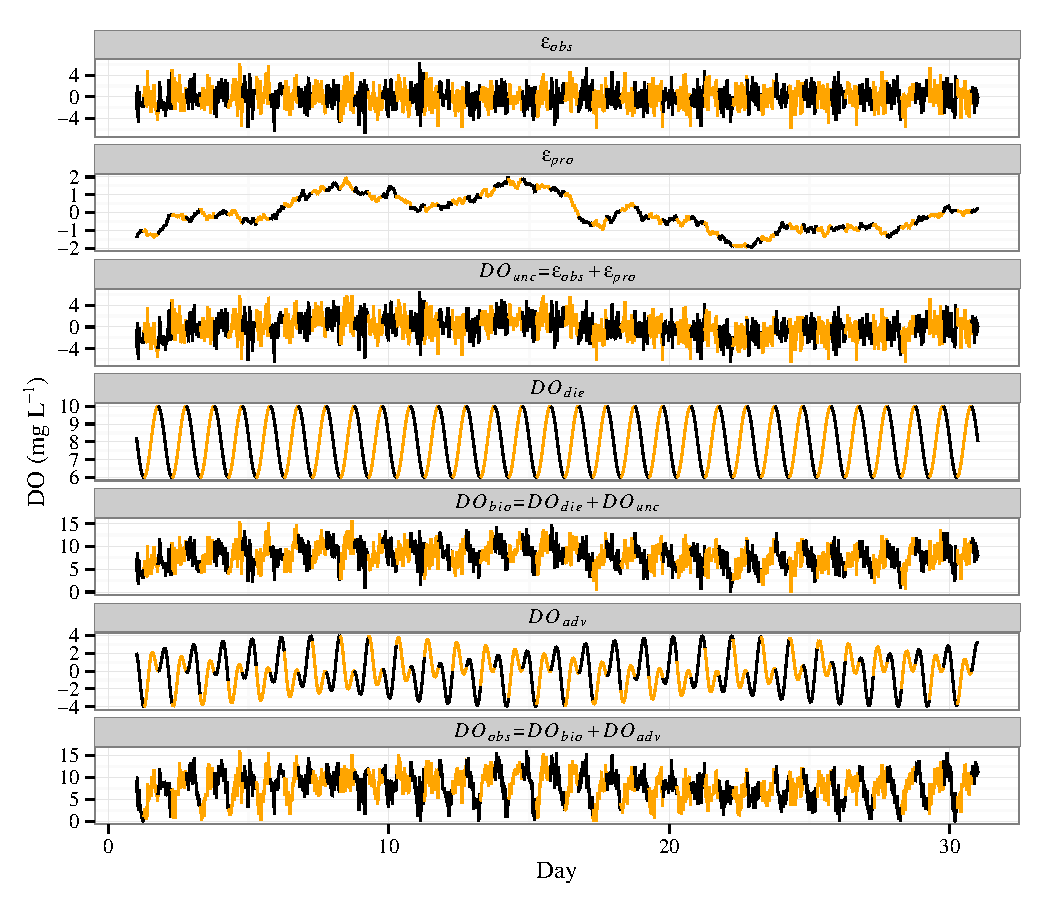
\includegraphics[width=\maxwidth]{figure/do_sim} 

}

\caption[Example of each component of a simulated \ac{DO} time series for testing weighted regression]{Example of each component of a simulated \ac{DO} time series for testing weighted regression.  The time series were created using \cref{do_obs,do_bio,do_unc,do_obs_all,do_sin,do_unc_n,deltdo,deltx,do_advp,do_adv}. Yellow indicates a twelve hour daylight period beginning at 630 each day.\label{fig:do_sim}}
\end{figure}


\end{knitrout}
\vfill
\clearpage

% plot of representative time series for simulation
\centering\vspace*{\fill}
\begin{knitrout}
\definecolor{shadecolor}{rgb}{0.969, 0.969, 0.969}\color{fgcolor}\begin{figure}[!ht]


{\centering 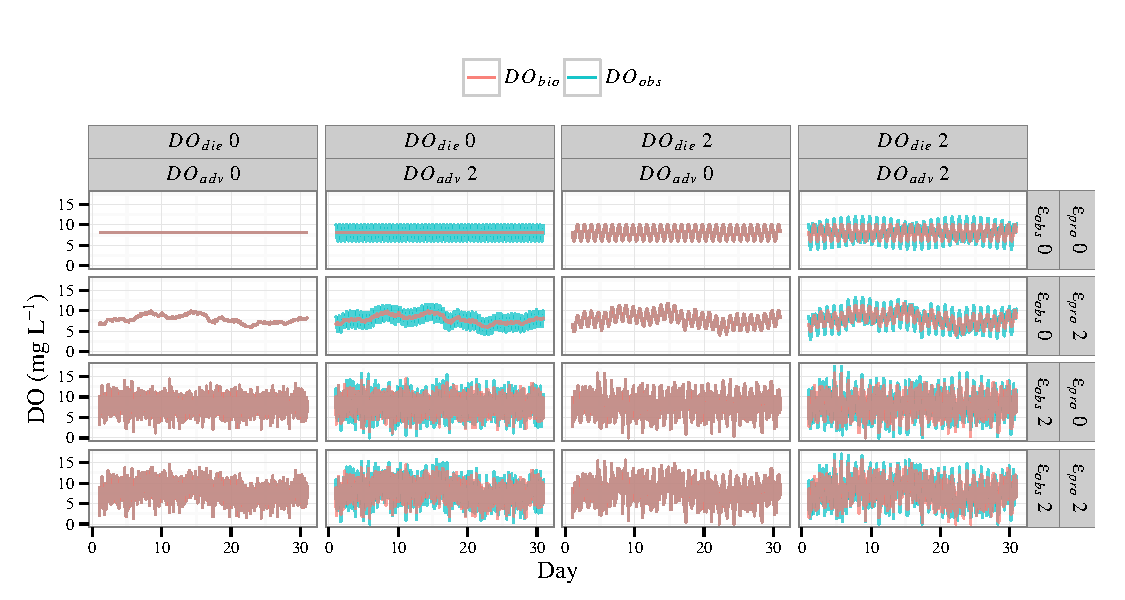
\includegraphics[width=\textwidth]{figure/sim_ex} 

}

\caption[Representative examples of simulated time series of observed \ac{DO} ($DO_{obs}$, blue lines) and biological \ac{DO} ($DO_{bio}$, as a component of observed, red lines) created by varying each of four parameters]{Representative examples of simulated time series of observed \ac{DO} ($DO_{obs}$, blue lines) and biological \ac{DO} ($DO_{bio}$, as a component of observed, red lines) created by varying each of four parameters: strength of tidal association with \ac{DO} signal ($DO_{adv}$), amount of process uncertainty ($\varepsilon_{pro}$), amount of observation uncertainty ($\varepsilon_{obs}$), and strength of diel \ac{DO} component ($DO_{die}$).  Parameter values represent the minimum and maximum used in the simulations as mg L$^{-1}$ of \ac{DO}.\label{fig:sim_ex}}
\end{figure}


\end{knitrout}
\vfill
\clearpage

% example of error surfaces 
\centering\vspace*{\fill}
\begin{knitrout}
\definecolor{shadecolor}{rgb}{0.969, 0.969, 0.969}\color{fgcolor}\begin{figure}[!ht]


{\centering 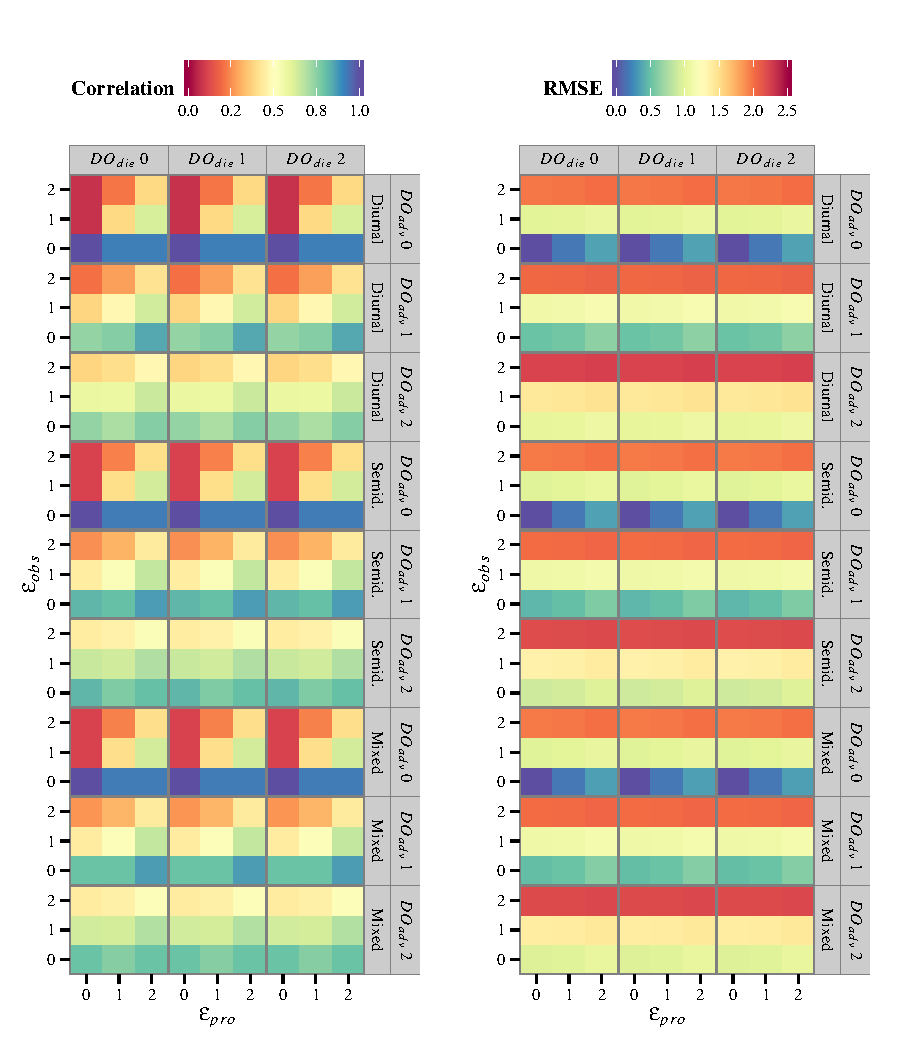
\includegraphics[width=\maxwidth]{figure/err_surf1} 

}

\caption[Heat maps of correlations and errors (\ac{RMSE}) for filtered \ac{DO} time series ($DO_{dtd}$) from weighted regression with `true' biological \ac{DO} ($DO_{bio}$) for varying simulation parameters]{Heat maps of correlations and errors (\ac{RMSE}) for filtered \ac{DO} time series ($DO_{dtd}$) from weighted regression with `true' biological \ac{DO} ($DO_{bio}$) for varying simulation parameters: strength of tidal association with \ac{DO} signal ($DO_{adv}$), amount of process uncertainty ($\varepsilon_{pro}$), amount of observation observation uncertainty ($\varepsilon_{obs}$), and strength of diel \ac{DO} component ($DO_{die}$).  Each tile represents the correlation or error from results for a given combination of simulation parameters averaged for all window widths (as in \cref{fig:err_surf2}).  See \cref{tab:dtd_perf1} for a summary of results for each unique parameter.\label{fig:err_surf1}}
\end{figure}


\end{knitrout}
\vfill
\clearpage

% example of error surfaces 
\centering\vspace*{\fill}
\begin{knitrout}
\definecolor{shadecolor}{rgb}{0.969, 0.969, 0.969}\color{fgcolor}\begin{figure}[!ht]


{\centering 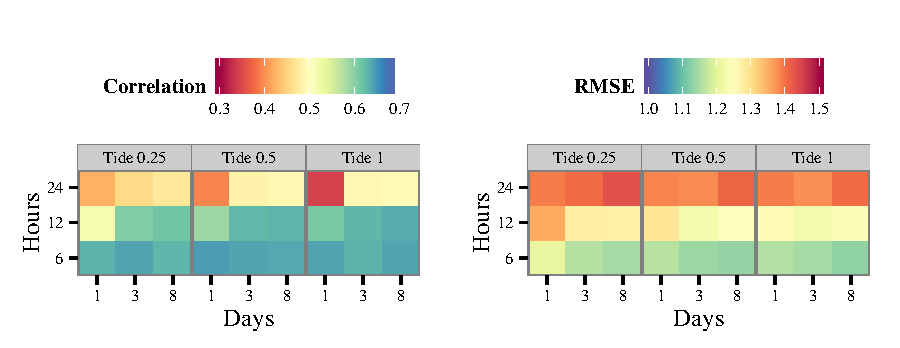
\includegraphics[width=\maxwidth]{figure/err_surf2} 

}

\caption[Heat maps of correlations and errors (\ac{RMSE}) for filtered \ac{DO} time series ($DO_{dtd}$) from weighted regression with `true' biological \ac{DO} ($DO_{bio}$) for varying half window widths]{Heat maps of correlations and errors (\ac{RMSE}) for filtered \ac{DO} time series ($DO_{dtd}$) from weighted regression with `true' biological \ac{DO} ($DO_{bio}$) for varying half window widths: days, hour of day, and proportion of tidal range.  Each tile represents the correlation or error from results for a given combination of window widths averaged for all simulation parameters (as in \cref{fig:err_surf1}).  See \cref{tab:dtd_perf2} for a summary of results for each unique window.\label{fig:err_surf2}}
\end{figure}


\end{knitrout}
\vfill
\clearpage

% maps of each case
\centering\vspace*{\fill}
\begin{knitrout}
\definecolor{shadecolor}{rgb}{0.969, 0.969, 0.969}\color{fgcolor}\begin{figure}[!ht]


{\centering 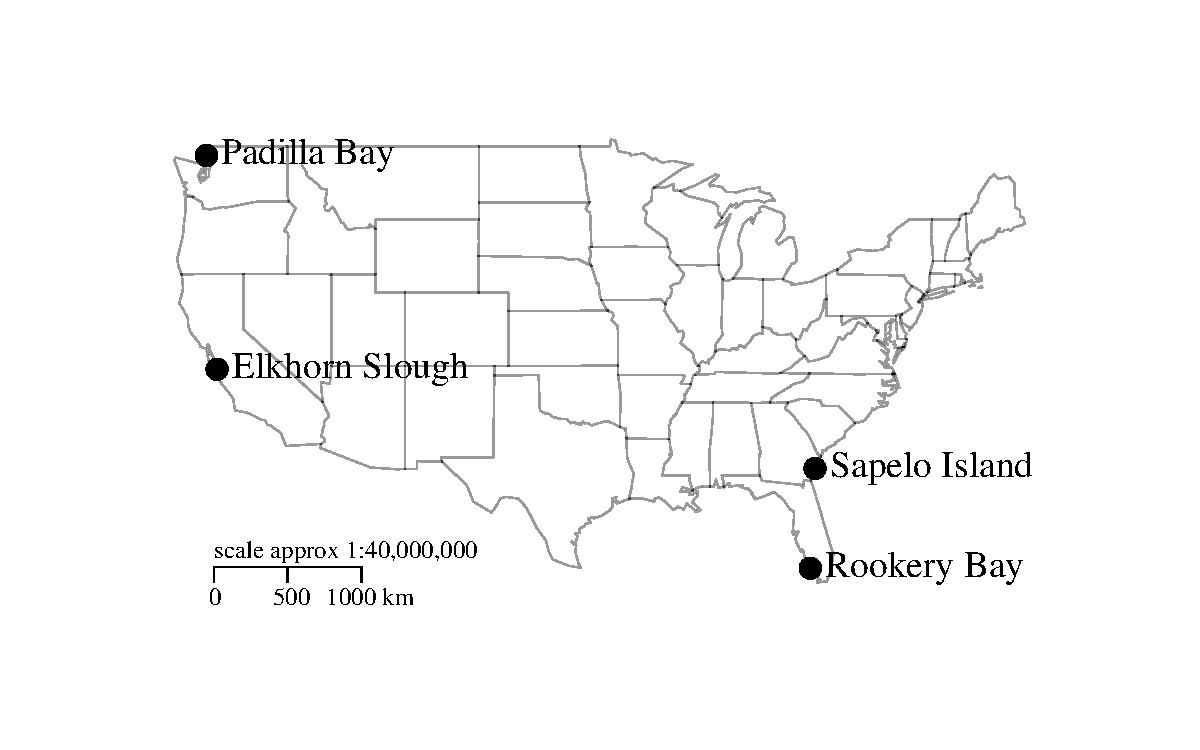
\includegraphics[width=\maxwidth]{figure/case_map} 

}

\caption[Locations of \ac{NERRS} sites used as case studies to validate weighted regression]{Locations of \ac{NERRS} sites used as case studies to validate weighted regression.  Stations at each reserve are ELKVM (Vierra Mouth at Elkhorn Slough), PDBBY (Bayview Channel at Padilla Bay), RKBMB (Middle Blackwater River at Rookery Bay), and SAPDC (Dean Creek at Sapelo Island).\label{fig:case_map}}
\end{figure}


\end{knitrout}
\vfill
\clearpage

% example from SAPHD, phase out
\centering\vspace*{\fill}
\begin{knitrout}
\definecolor{shadecolor}{rgb}{0.969, 0.969, 0.969}\color{fgcolor}\begin{figure}[!ht]


{\centering 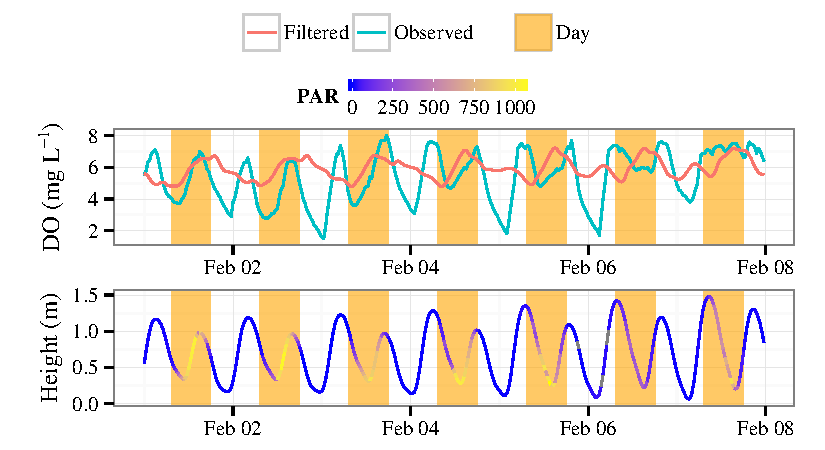
\includegraphics[width=0.8\textwidth]{figure/phase_out} 

}

\caption[Continuous \ac{DO} time series before (observed) and after (filtered) filtering with weighted regression (top) and tidal height (m) colored by total photosynthetically active radiation (bottom, mmol m$^{-2}$)]{Continuous \ac{DO} time series before (observed) and after (filtered) filtering with weighted regression (top) and tidal height (m) colored by total photosynthetically active radiation (bottom, mmol m$^{-2}$). Results are for the Sapelo Island station for a seven day period when high tide events were out of phase with diel periods, creating lower than expected observed \ac{DO} during night and day periods. Filtered values are based on a weighted regression with half window widths of six days, one hour within each day, and tidal height proportion of one half.\label{fig:phase_out}}
\end{figure}


\end{knitrout}
\vfill
\clearpage

% example from SAPHD, phase in
\centering\vspace*{\fill}
\begin{knitrout}
\definecolor{shadecolor}{rgb}{0.969, 0.969, 0.969}\color{fgcolor}\begin{figure}[!ht]


{\centering 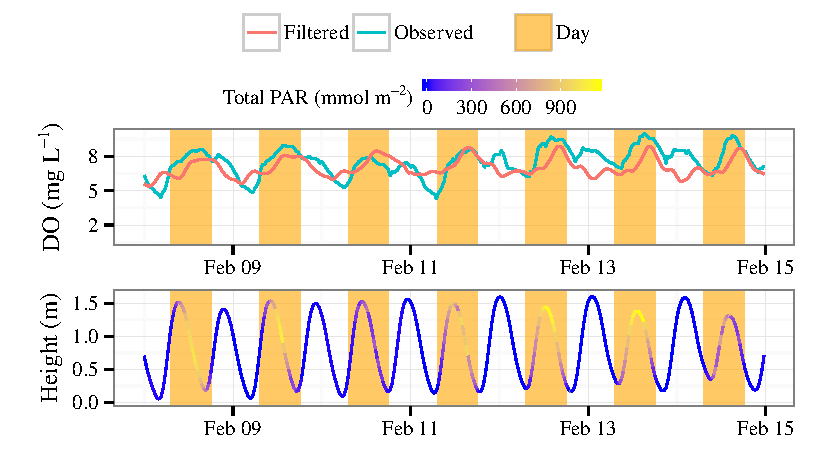
\includegraphics[width=0.8\textwidth]{figure/phase_in} 

}

\caption[Continuous \ac{DO} time series before (observed) and after (filtered) filtering with weighted regression (top) and tidal height (m) colored by total photosynthetically active radiation (bottom, mmol m$^{-2}$)]{Continuous \ac{DO} time series before (observed) and after (filtered) filtering with weighted regression (top) and tidal height (m) colored by total photosynthetically active radiation (bottom, mmol m$^{-2}$). Results are for the Sapelo Island station for a seven day period when high tide events were in phase with diel periods, creating higher than expected observed \ac{DO} during night and day periods. Filtered values are based on a weighted regression with half window widths of six days, one hour within each day, and tidal height proportion of one half.\label{fig:phase_in}}
\end{figure}


\end{knitrout}
\vfill
\clearpage

% example from SAPDC
\centering\vspace*{\fill}
\begin{knitrout}
\definecolor{shadecolor}{rgb}{0.969, 0.969, 0.969}\color{fgcolor}\begin{figure}[!ht]


{\centering 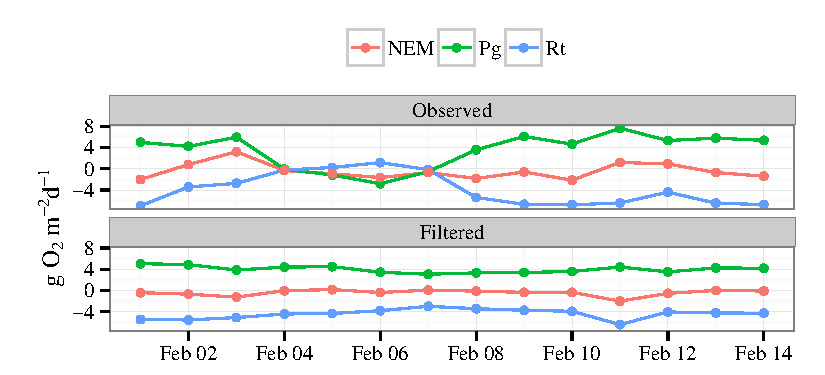
\includegraphics[width=0.8\textwidth]{figure/case_ex} 

}

\caption[Example of daily mean metabolism (net ecosystem metabolism, gross production, and total respiration) before (observed) and after (filtered) filtering with weighted regression]{Example of daily mean metabolism (net ecosystem metabolism, gross production, and total respiration) before (observed) and after (filtered) filtering with weighted regression. Results are for the Sapelo Island station for a two week period in February, 2012 when high tide was out of phase with the diel cycle during the first week (\cref{fig:phase_out}) and in phase during the second week (\cref{fig:phase_in}).\label{fig:case_ex}}
\end{figure}


\end{knitrout}

% moving correlations
\centering\vspace*{\fill}
\begin{knitrout}
\definecolor{shadecolor}{rgb}{0.969, 0.969, 0.969}\color{fgcolor}\begin{figure}[!ht]


{\centering 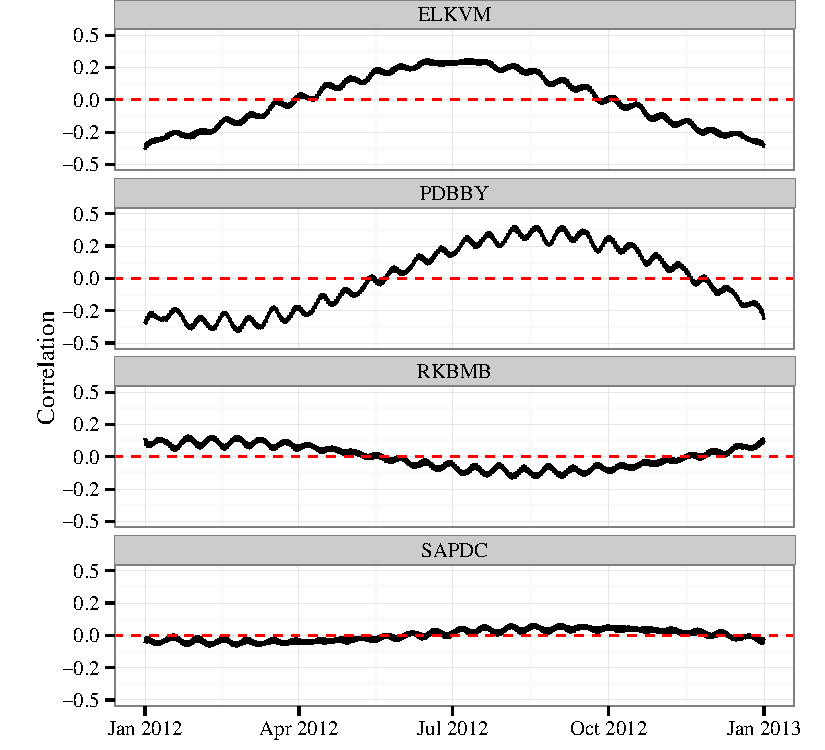
\includegraphics[width=0.8\textwidth]{figure/move_corrs} 

}

\caption[Correlations of sun angle with tidal change (as an angular rate) using a half-window width of 12 days]{Correlations of sun angle with tidal change (as an angular rate) using a half-window width of 12 days.  Correlations larger or smaller than zero are periods when weighted regression may not effectively quantify variation from biological and physical sources in \ac{DO} time series due to collinearity.\label{fig:move_corrs}}
\end{figure}


\end{knitrout}

% plots of summarized metabolism estimates, before/after detiding
% all case studies
\centering\vspace*{\fill}
\begin{knitrout}
\definecolor{shadecolor}{rgb}{0.969, 0.969, 0.969}\color{fgcolor}\begin{figure}[!ht]


{\centering 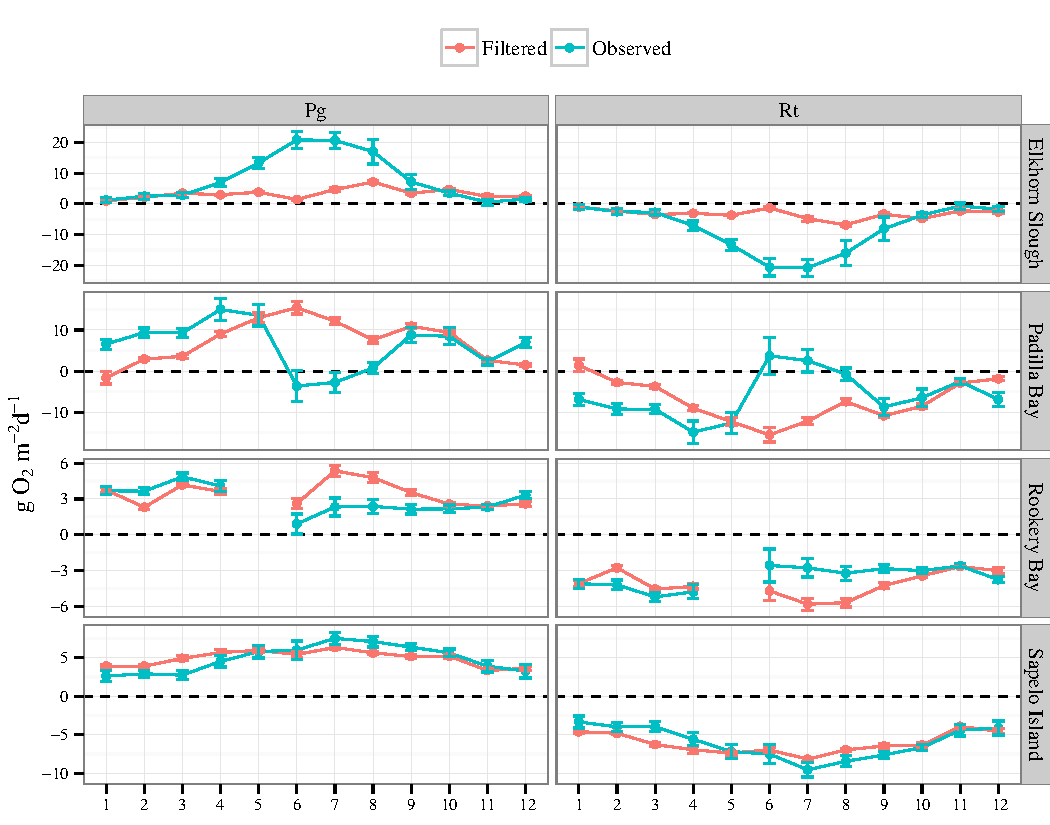
\includegraphics[width=\maxwidth]{figure/metab_sum} 

}

\caption[Means and standard errors of daily metabolism estimates (gross production, total respiration) aggregated by month]{Means and standard errors of daily metabolism estimates (gross production, total respiration) aggregated by month.  Aggregated estimates are shown for observed and filtered \ac{DO} time series.  May was removed from Rookery Bay because of incomplete data.\label{fig:metab_sum}}
\end{figure}


\end{knitrout}
\vfill
\clearpage

%%%%%%
% tables

\section{Tables}

% summary of simulation performance for detided and biological, sim parameters
%latex.default(tab, file = "", where = "h", rowlabel = "Parameter",     caption = cap.val, caption.loc = "top", rgroup = Parms, n.rgroup = rep(3,         4), cgroup = c("Correlation", "RMSE"), n.cgroup = c(5,         5), rowname = rows, colheads = rep(c("Min", "25\\textsuperscript{th}",         "Median", "75\\textsuperscript{th}", "Max"), 2), label = "tab:dtd_perf1")%
\begin{table}[h]
\caption{Summary (range, median, quartiles) of correlations and error estimates comparing filtered and biological \ac{DO} time series for different simulation parameters ($DO_{die}$, $DO_{adv}$, $\varepsilon_{pro}$, $\varepsilon_{obs}$).  Values represent averages from multiple simulations with common parameters.  For example, row one is a summary of all simulations for which the diel \ac{DO} component was zero ($n=729$).  See \cref{fig:err_surf1} for results of all parameter combinations.\label{tab:dtd_perf1}} 
\begin{center}
\begin{tabular}{llllllclllll}
\hline\hline
\multicolumn{1}{l}{\bfseries Parameter}&\multicolumn{5}{c}{\bfseries Correlation}&\multicolumn{1}{c}{\bfseries }&\multicolumn{5}{c}{\bfseries RMSE}\tabularnewline
\cline{2-6} \cline{8-12}
\multicolumn{1}{l}{}&\multicolumn{1}{c}{Min}&\multicolumn{1}{c}{25\textsuperscript{th}}&\multicolumn{1}{c}{Median}&\multicolumn{1}{c}{75\textsuperscript{th}}&\multicolumn{1}{c}{Max}&\multicolumn{1}{c}{}&\multicolumn{1}{c}{Min}&\multicolumn{1}{c}{25\textsuperscript{th}}&\multicolumn{1}{c}{Median}&\multicolumn{1}{c}{75\textsuperscript{th}}&\multicolumn{1}{c}{Max}\tabularnewline
\hline
{\bfseries $\boldsymbol{DO_{die}}$}&&&&&&&&&&&\tabularnewline
~~0&0.05&0.20&0.41&0.86&1.00&&0.00&0.33&1.01&1.96&2.05\tabularnewline
~~1&0.28&0.44&0.61&0.93&1.00&&0.02&0.42&1.02&1.96&2.06\tabularnewline
~~2&0.55&0.60&0.81&0.96&1.00&&0.05&0.52&1.06&1.99&2.12\tabularnewline
\hline
{\bfseries $\boldsymbol{DO_{adv}}$}&&&&&&&&&&&\tabularnewline
~~0&0.05&0.42&0.63&0.93&1.00&&0.00&0.46&1.02&1.97&2.12\tabularnewline
~~1&0.05&0.42&0.63&0.93&1.00&&0.00&0.46&1.02&1.97&2.12\tabularnewline
~~2&0.05&0.42&0.63&0.93&1.00&&0.00&0.46&1.02&1.97&2.12\tabularnewline
\hline
{\bfseries $\boldsymbol{\varepsilon_{pro}}$}&&&&&&&&&&&\tabularnewline
~~0&0.05&0.31&0.58&0.99&1.00&&0.00&0.23&0.99&1.95&2.11\tabularnewline
~~1&0.16&0.37&0.61&0.93&0.99&&0.10&0.33&1.02&1.97&2.11\tabularnewline
~~2&0.34&0.58&0.69&0.89&0.98&&0.19&0.56&1.10&2.01&2.12\tabularnewline
\hline
{\bfseries $\boldsymbol{\varepsilon_{obs}}$}&&&&&&&&&&&\tabularnewline
~~0&0.80&0.93&0.97&0.99&1.00&&0.00&0.17&0.29&0.46&0.84\tabularnewline
~~1&0.05&0.56&0.62&0.81&0.84&&0.97&1.00&1.02&1.08&1.28\tabularnewline
~~2&0.05&0.31&0.38&0.57&0.63&&1.93&1.97&1.98&2.01&2.12\tabularnewline
\hline
\end{tabular}\end{center}

\end{table}


% summary of simulation performance for detided and biological, window widths
%latex.default(tab, file = "", rowlabel = "Window", caption = cap.val,     caption.loc = "top", rgroup = Parms, n.rgroup = rep(3, 3),     cgroup = c("Correlation", "RMSE"), n.cgroup = c(5, 5), rowname = rows,     colheads = rep(c("Min", "25\\textsuperscript{th}", "Median",         "75\\textsuperscript{th}", "Max"), 2), label = "tab:dtd_perf2")%
\begin{table}[!tbp]
\caption{Summary (range, median, quartiles) of correlations and error estimates comparing filtered and biological \ac{DO} time series for simulations using different half window widths in the weighted regressions (days, hours, and proportion of tidal range).  Values represent averages from multiple simulations with common window values For example, row one is a summary of all simulations for which the half window width was one day ($n=729$). See \cref{fig:err_surf2} for results of all window combinations.\label{tab:dtd_perf2}} 
\begin{center}
\begin{tabular}{llllllclllll}
\hline\hline
\multicolumn{1}{l}{\bfseries Window}&\multicolumn{5}{c}{\bfseries Correlation}&\multicolumn{1}{c}{\bfseries }&\multicolumn{5}{c}{\bfseries RMSE}\tabularnewline
\cline{2-6} \cline{8-12}
\multicolumn{1}{l}{}&\multicolumn{1}{c}{Min}&\multicolumn{1}{c}{25\textsuperscript{th}}&\multicolumn{1}{c}{Median}&\multicolumn{1}{c}{75\textsuperscript{th}}&\multicolumn{1}{c}{Max}&\multicolumn{1}{c}{}&\multicolumn{1}{c}{Min}&\multicolumn{1}{c}{25\textsuperscript{th}}&\multicolumn{1}{c}{Median}&\multicolumn{1}{c}{75\textsuperscript{th}}&\multicolumn{1}{c}{Max}\tabularnewline
\hline
{\bfseries Days}&&&&&&&&&&&\tabularnewline
~~1&0.07&0.44&0.66&0.96&1.00&&0.00&0.43&1.02&1.96&2.12\tabularnewline
~~3&0.07&0.41&0.62&0.93&1.00&&0.00&0.45&1.02&1.97&2.08\tabularnewline
~~6&0.05&0.37&0.61&0.88&1.00&&0.00&0.51&1.02&1.97&2.08\tabularnewline
\hline
{\bfseries Hours}&&&&&&&&&&&\tabularnewline
~~1&0.07&0.38&0.61&0.89&1.00&&0.00&0.51&1.02&1.97&2.05\tabularnewline
~~3&0.06&0.42&0.63&0.95&1.00&&0.00&0.43&1.02&1.97&2.05\tabularnewline
~~6&0.05&0.44&0.64&0.95&1.00&&0.00&0.48&1.04&1.96&2.12\tabularnewline
\hline
{\bfseries Tide}&&&&&&&&&&&\tabularnewline
~~0.25&0.05&0.42&0.62&0.92&1.00&&0.00&0.47&1.03&1.97&2.12\tabularnewline
~~0.5&0.07&0.42&0.63&0.94&1.00&&0.00&0.45&1.02&1.96&2.04\tabularnewline
~~1&0.07&0.42&0.63&0.94&1.00&&0.00&0.44&1.02&1.97&2.04\tabularnewline
\hline
\end{tabular}\end{center}

\end{table}


% descriptive table of case studies
%latex.default(tab, file = "", rowlabel = "Site", insert.bottom = foot.val,     caption = cap.val, caption.loc = "top", cgroup = c("Tidal amplitude",         "Water quality", "Metabolism\\textsuperscript{\\textit{a}}"),     n.cgroup = c(4, 4, 3), rowname = rows, colheads = c("O1",         "P1", "M2", "S2", "DO", "Chl", "Sal", "Temp", "Pg", "Rt",         "NEM"), label = "tab:case_att")%
\begin{table}[!tbp]
\caption{Summary statistics of tidal component amplitudes (m), selected water quality parameters (\ac{DO} mg L$^{-1}$, chlorophyll-a $\mu$g L$^{-1}$, salinity psu, water temperature $^{\circ}$C)  and metabolism estimates (gross production, respiration, and net ecosystem metabolism as g m$^{-2}$ d$^{-1}$ based on observed data) for each case study.  Tidal components are principal lunar semidiurnal (O1, frequency 25.82 hours), solar diurnal (P1, 24.07 hours), lunar semidiurnal (M2, 12.42 hours), and solar semidiurnal (S2, 12 hours) estimated from harmonic regressions of tidal height (\texttt{oce} package in R, \citealt{Foreman89}, \citetalias{RDCT14}).  Water quality data are averages for the entire period of record for each site.  Metabolism estimates are means of daily integrated values.\label{tab:case_att}} 
\begin{center}
\begin{tabular}{lllllcllllclll}
\hline\hline
\multicolumn{1}{l}{\bfseries Site}&\multicolumn{4}{c}{\bfseries Tidal amplitude}&\multicolumn{1}{c}{\bfseries }&\multicolumn{4}{c}{\bfseries Water quality}&\multicolumn{1}{c}{\bfseries }&\multicolumn{3}{c}{\bfseries Metabolism\textsuperscript{\textit{a}}}\tabularnewline
\cline{2-5} \cline{7-10} \cline{12-14}
\multicolumn{1}{l}{}&\multicolumn{1}{c}{O1}&\multicolumn{1}{c}{P1}&\multicolumn{1}{c}{M2}&\multicolumn{1}{c}{S2}&\multicolumn{1}{c}{}&\multicolumn{1}{c}{DO}&\multicolumn{1}{c}{Chl}&\multicolumn{1}{c}{Sal}&\multicolumn{1}{c}{Temp}&\multicolumn{1}{c}{}&\multicolumn{1}{c}{Pg}&\multicolumn{1}{c}{Rt}&\multicolumn{1}{c}{NEM}\tabularnewline
\hline
ELKVM&0.24&0.12&0.48&0.13&&7.87&3.87&32.43&13.78&&8.14&-8.19&-0.05\tabularnewline
PDBBY&0.46&0.23&0.63&0.15&&8.97&2.24&29.17&10.44&&5.95&-5.90& 0.05\tabularnewline
RKBMB&0.13&0.04&0.36&0.10&&4.48&4.50&30.53&25.85&&3.02&-3.62&-0.60\tabularnewline
SAPDC&0.10&0.02&0.54&0.07&&4.96&5.98&27.30&21.77&&4.89&-6.04&-1.16\tabularnewline
\hline
\end{tabular}\end{center}

\footnotesize\textsuperscript{\textit{a}}Pg: gross production, Rt: respiration, NEM: net ecosystem metabolism, estimated using methods described herein with observed data\end{table}


% correlations with tide before/after wtreg
%latex.default(tab, file = "", rowlabel = "Site", rgroup = unique(rows),     n.rgroup = rep(2, 4), insert.bottom = foot.val, caption = cap.val,     colheads = c("DO", "Pg\\textsuperscript{\\textit{a}}", "Rt"),     caption.loc = "top", rowname = rep(c("Observed", "Filtered"),         4), label = "tab:cor_res")%
\begin{table}[!tbp]
\caption{Correlations of tidal changes at each site with continuous \ac{DO} observations and metabolism estimates (gross production, respiration) before (observed) and after (filtered) filtering with weighted regression.  Values are averages of monthly correlations.  \ac{DO} values are correlated with predicted tidal height at each observation, whereas metabolism estimates are correlated with mean tidal height change between observations during day or night periods for production and respiration, respectively.\label{tab:cor_res}} 
\begin{center}
\begin{tabular}{llll}
\hline\hline
\multicolumn{1}{l}{Site}&\multicolumn{1}{c}{DO}&\multicolumn{1}{c}{Pg\textsuperscript{\textit{a}}}&\multicolumn{1}{c}{Rt}\tabularnewline
\hline
{\bfseries ELKVM}&&&\tabularnewline
~~Observed& 0.44& 0.43& 0.43\tabularnewline
~~Filtered&-0.04& 0.04&-0.01\tabularnewline
\hline
{\bfseries PDBBY}&&&\tabularnewline
~~Observed&-0.49&-0.11&-0.29\tabularnewline
~~Filtered& 0.01&-0.05& 0.00\tabularnewline
\hline
{\bfseries RKBMB}&&&\tabularnewline
~~Observed& 0.45& 0.26& 0.34\tabularnewline
~~Filtered& 0.02&-0.04& 0.03\tabularnewline
\hline
{\bfseries SAPDC}&&&\tabularnewline
~~Observed& 0.62& 0.47& 0.64\tabularnewline
~~Filtered& 0.00&-0.04& 0.07\tabularnewline
\hline
\end{tabular}\end{center}

\textsuperscript{\textit{a}}Pg: gross production, Rt: respiration, NEM: net ecosystem metabolism\end{table}


% case study metabolism results, including perc anom
%latex.default(tab, file = "", rowlabel = "Site", insert.bottom = foot.val,     caption = cap.val, caption.loc = "top", rgroup = unique(to_tab$Site),     n.rgroup = rep(2, 4), cgroup = c("Pg\\textsuperscript{\\textit{a}}",         "Rt"), n.cgroup = c(3, 3), rowname = rows, colheads = c(rep(c("Mean",         "SD", "Anom"), 2), c("Mean", "SD")), label = "tab:case_res")%
\begin{table}[!tbp]
\caption{Summary of metabolism estimates (gross production, respiration) for case studies using \ac{DO} time series before (observed) and after (filtered) filtering with weighted regression.  Means and standard deviation are based on daily integrated metabolism estimates.  Anomalous values are the percentage of metabolism estimates that were negative for gross production and positive for respiration.\label{tab:case_res}} 
\begin{center}
\begin{tabular}{llllclll}
\hline\hline
\multicolumn{1}{l}{\bfseries Site}&\multicolumn{3}{c}{\bfseries Pg\textsuperscript{\textit{a}}}&\multicolumn{1}{c}{\bfseries }&\multicolumn{3}{c}{\bfseries Rt}\tabularnewline
\cline{2-4} \cline{6-8}
\multicolumn{1}{l}{}&\multicolumn{1}{c}{Mean}&\multicolumn{1}{c}{SD}&\multicolumn{1}{c}{Anom}&\multicolumn{1}{c}{}&\multicolumn{1}{c}{Mean}&\multicolumn{1}{c}{SD}&\multicolumn{1}{c}{Anom}\tabularnewline
\hline
{\bfseries ELKVM}&&&&&&&\tabularnewline
~~Observed&8.14&11.44&18.64&&-8.19&11.82&20.68\tabularnewline
~~Filtered&3.00& 2.26& 6.78&&-3.06& 2.34& 7.12\tabularnewline
\hline
{\bfseries PDBBY}&&&&&&&\tabularnewline
~~Observed&5.95&11.69&21.80&&-5.90&12.60&19.03\tabularnewline
~~Filtered&7.01& 6.85& 4.84&&-7.01& 6.81& 5.54\tabularnewline
\hline
{\bfseries RKBMB}&&&&&&&\tabularnewline
~~Observed&3.02& 2.55& 9.15&&-3.62& 2.65& 7.57\tabularnewline
~~Filtered&3.46& 1.79& 0.63&&-4.07& 1.88& 0.63\tabularnewline
\hline
{\bfseries SAPDC}&&&&&&&\tabularnewline
~~Observed&4.89& 4.42&13.39&&-6.04& 4.78&10.93\tabularnewline
~~Filtered&4.94& 1.74& 0.00&&-6.13& 1.99& 0.00\tabularnewline
\hline
\end{tabular}\end{center}

\textsuperscript{\textit{a}}Pg: gross production, Rt: respiration\end{table}


\clearpage

%%%%%%
% multimedia files, appendices

\raggedbottom
\raggedright
\setlength{\parindent}{0.5in}

\section{Multimedia} \label{multi}
The supporting information for this manuscript includes a graphical illustration of the weighting scheme described in the material and procedures section (\href{http://spark.rstudio.com/beckmw/weights_widget}{http://spark.rstudio.com/beckmw/weights\_widget}), results for each simulation (\href{http://spark.rstudio.com/beckmw/detiding_sims}{http://spark.rstudio.com/beckmw/detiding\_sims}), and results for each case study (\href{http://spark.rstudio.com/beckmw/detiding_cases}{http://spark.rstudio.com/beckmw/detiding\_cases}).  Each link is a graphical summary of data based on interactive inputs to support the results in the manuscript.

A simple R package with a sample dataset and code to implement weighted regression is also available on GitHub.  Functions are also availabe to estimate ecosystem metabolism.  See the README file on the web page for download instructions and examples: \href{https://github.com/fawda123/WtRegDO}{https://github.com/fawda123/WtRegDO}

\end{document}
